\section{The Ising model}


\begin{figure}[H]
  \begin{center}
    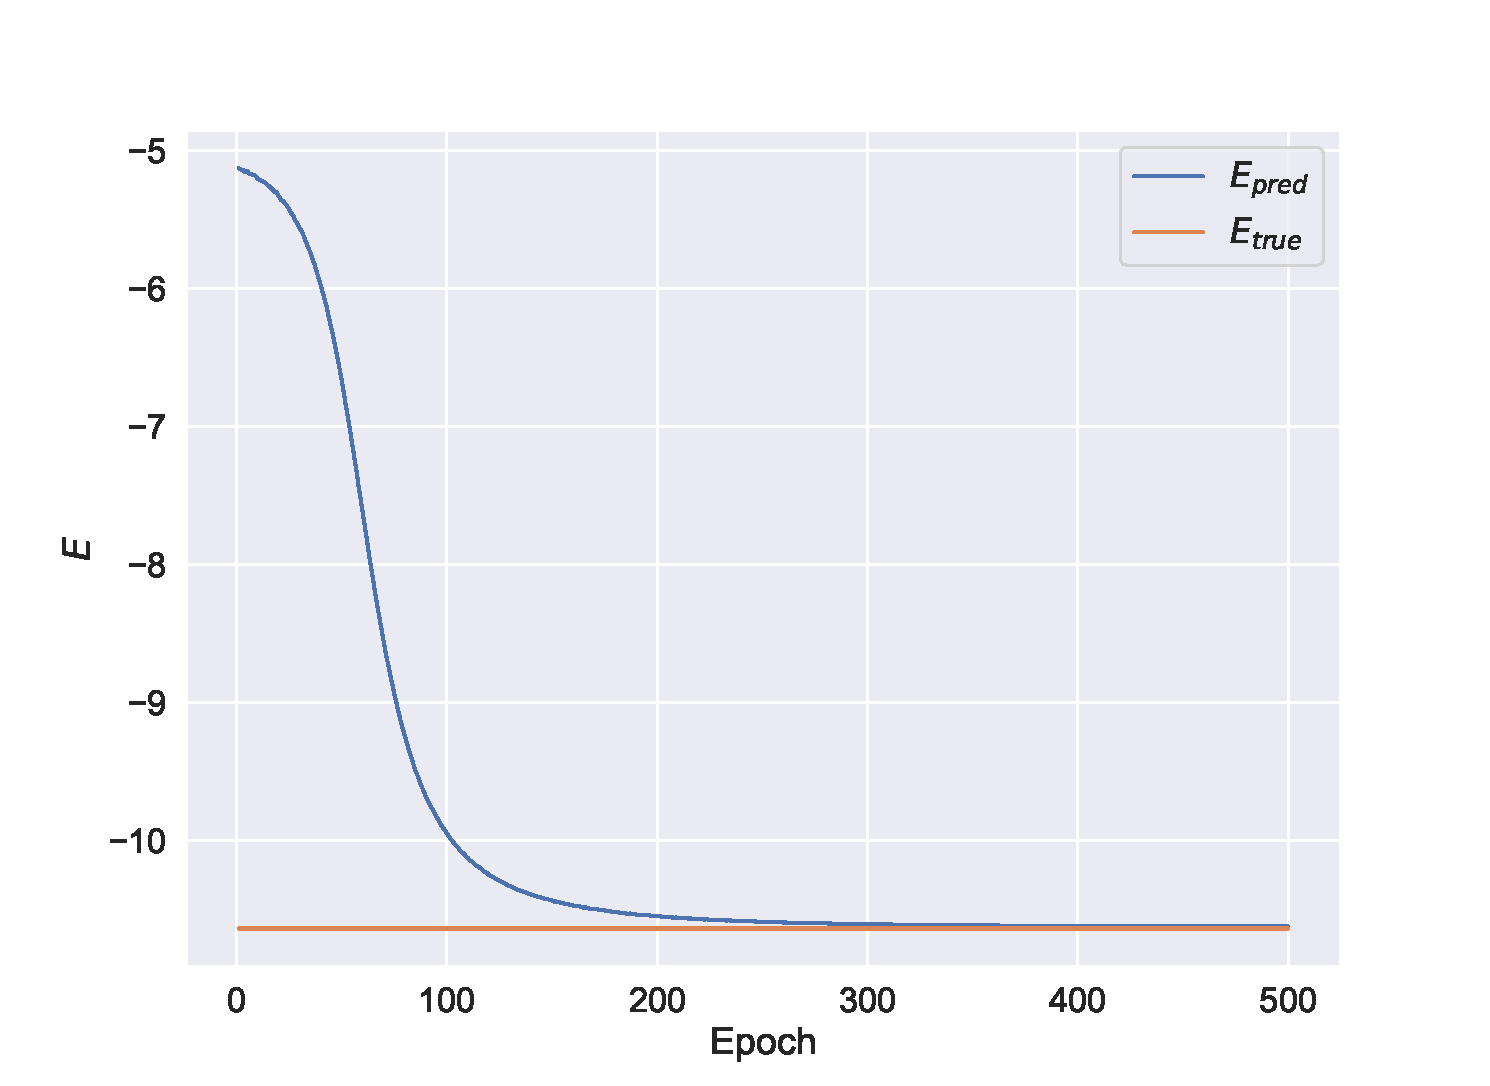
\includegraphics[width=0.95\textwidth]{Figures/Plots/Ising/ising_conv10}
  \end{center}
  \caption{The convergence graph of the RBM mean energy output for the Ising model with $N = 14$ particles, $M=1$, and $J=-1$ and $L=-0.5$.}
\end{figure}

The two-dimensional Ising model results in the following convergence graph:

\begin{figure}[H]
  \begin{center}
    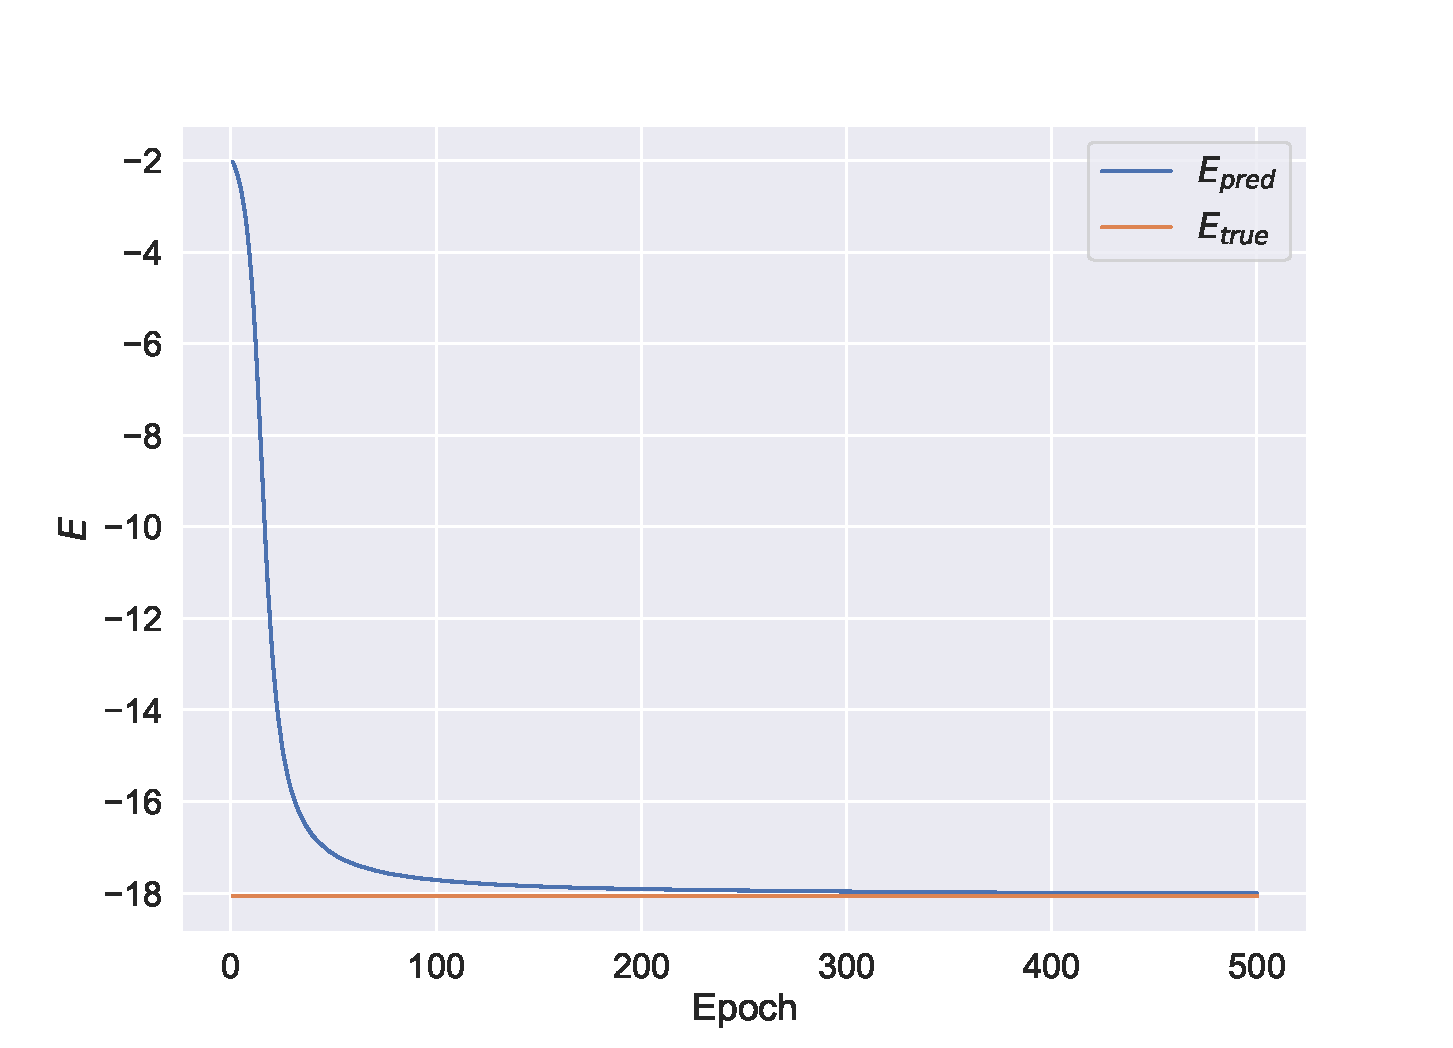
\includegraphics[width=0.95\textwidth]{Figures/Plots/Ising/ising_conv33}
  \end{center}
  \caption{The convergence graph of the RBM mean energy output for the two-dimensional Ising model with $N = 3$ particles, $M=3$, and $J=-1$ and $L=-0.5$.}
\end{figure}

\subsection{The effect of \texorpdfstring{$J$}{J} on RBM prediction accuracy}

For one dimensions and with the external field $L=-0.5$, we get
\begin{figure}[H]
  \begin{center}
    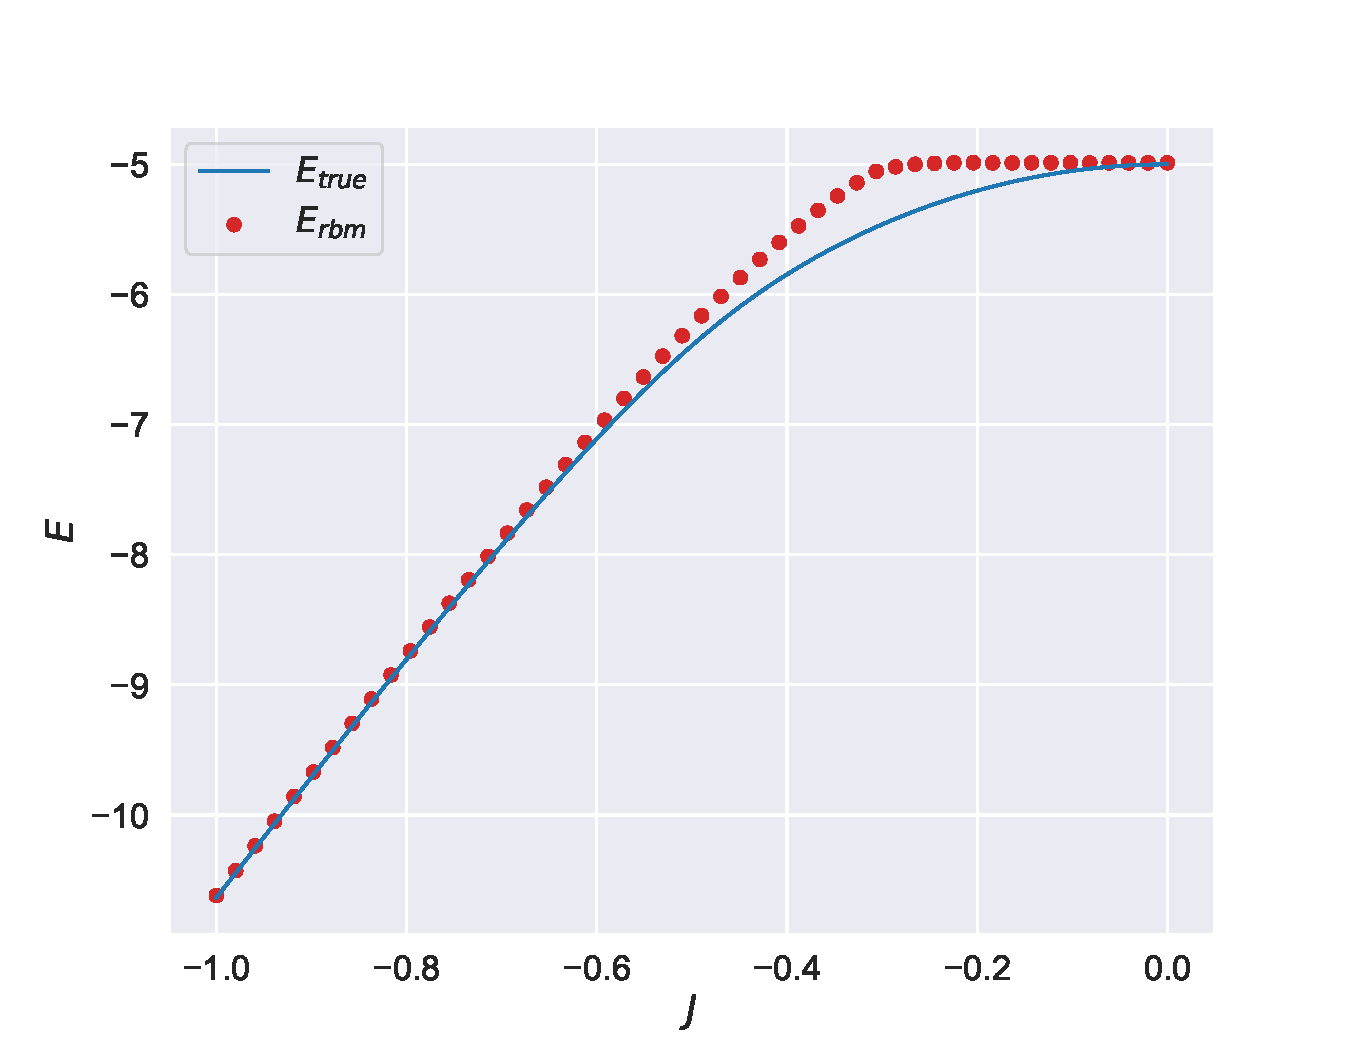
\includegraphics[width=0.95\textwidth]{Figures/Plots/Ising/val-true[J][-1.0-0.0][e=500][n=10][L=-0.5]}
  \end{center}
  \caption{The true ground state energy together with the restricted Boltzmann machine local energy output for the Ising model with $10$ lattice points and $L=-0.5$.}
\end{figure}

The RBM manges fine until about $J=-0.4$ where it snaps up to $-5$. If we check the two-dimensional case as well:

\begin{figure}[H]
  \begin{center}
    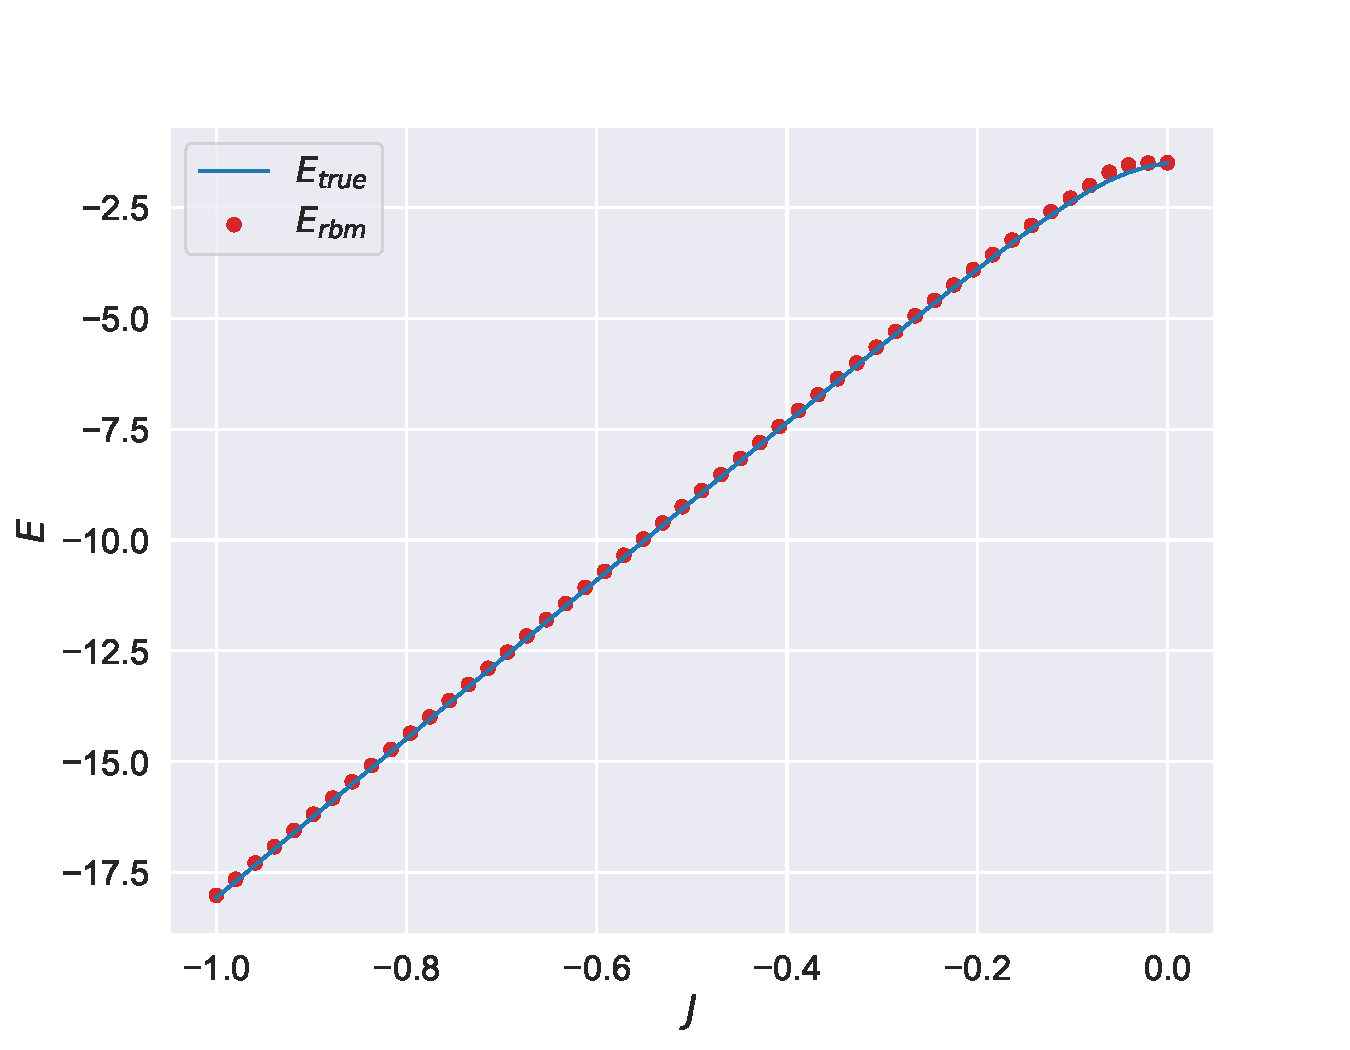
\includegraphics[width=0.95\textwidth]{Figures/Plots/Ising/val-true[J][-1.0-0.0][e=500][n=9][L=-0.5]}
  \end{center} 
  \caption{The true ground state energy together with the restricted Boltzmann machine local energy output for the two-dimensional Ising model with $9$ lattice points, $N=3$ and $M=3$, and $L=-0.5$.}
\end{figure}

Here the RBM manages to predict with higher accuracy, though we still see a small increase in error closer towards zero. A possible explanation could be that the RBM defaults to the non-interactive state as the interaction strength becomes small enough.

\subsection{The effect of \texorpdfstring{$L$}{L} on RBM prediction accuracy}

\begin{figure}[H]
  \begin{center}
    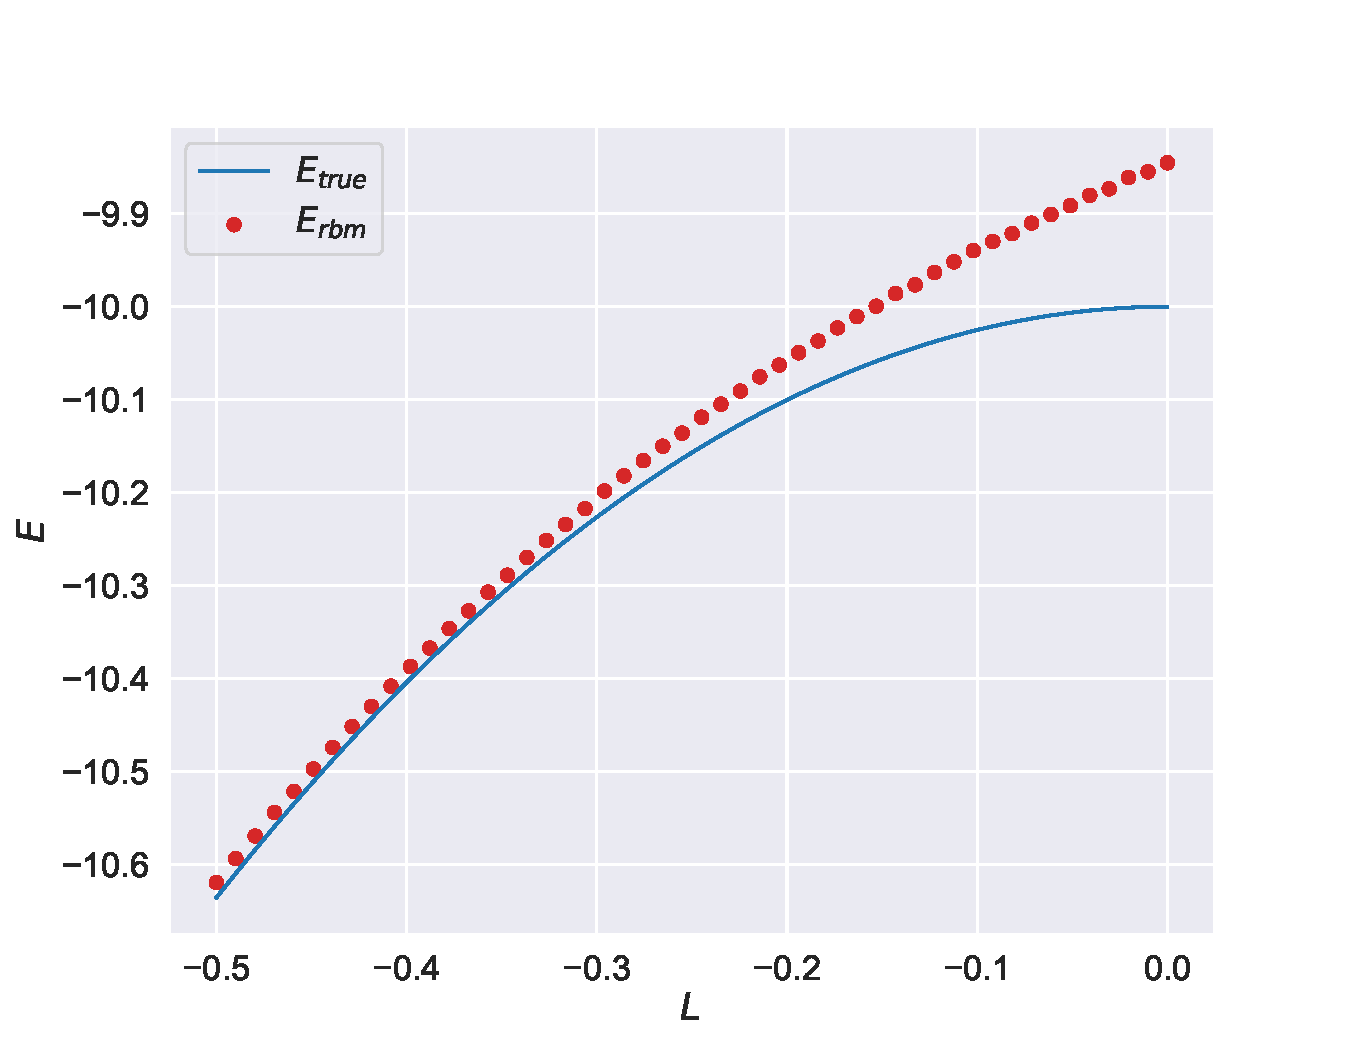
\includegraphics[width=0.95\textwidth]{Figures/Plots/Ising/val-true[L][-0.5-0.0][e=500][n=10][J=-1]}
  \end{center}
  \caption{The true ground state energy together with the restricted Boltzmann machine local energy output for the Ising model with $10$ lattice points and $J=-1$.}
\end{figure}

The RBM manages to approximate the ground state energy well up to about $L = -0.3$, where it suddenly diverges from the true value. With two dimensions we get:

\begin{figure}[H]
  \begin{center}
    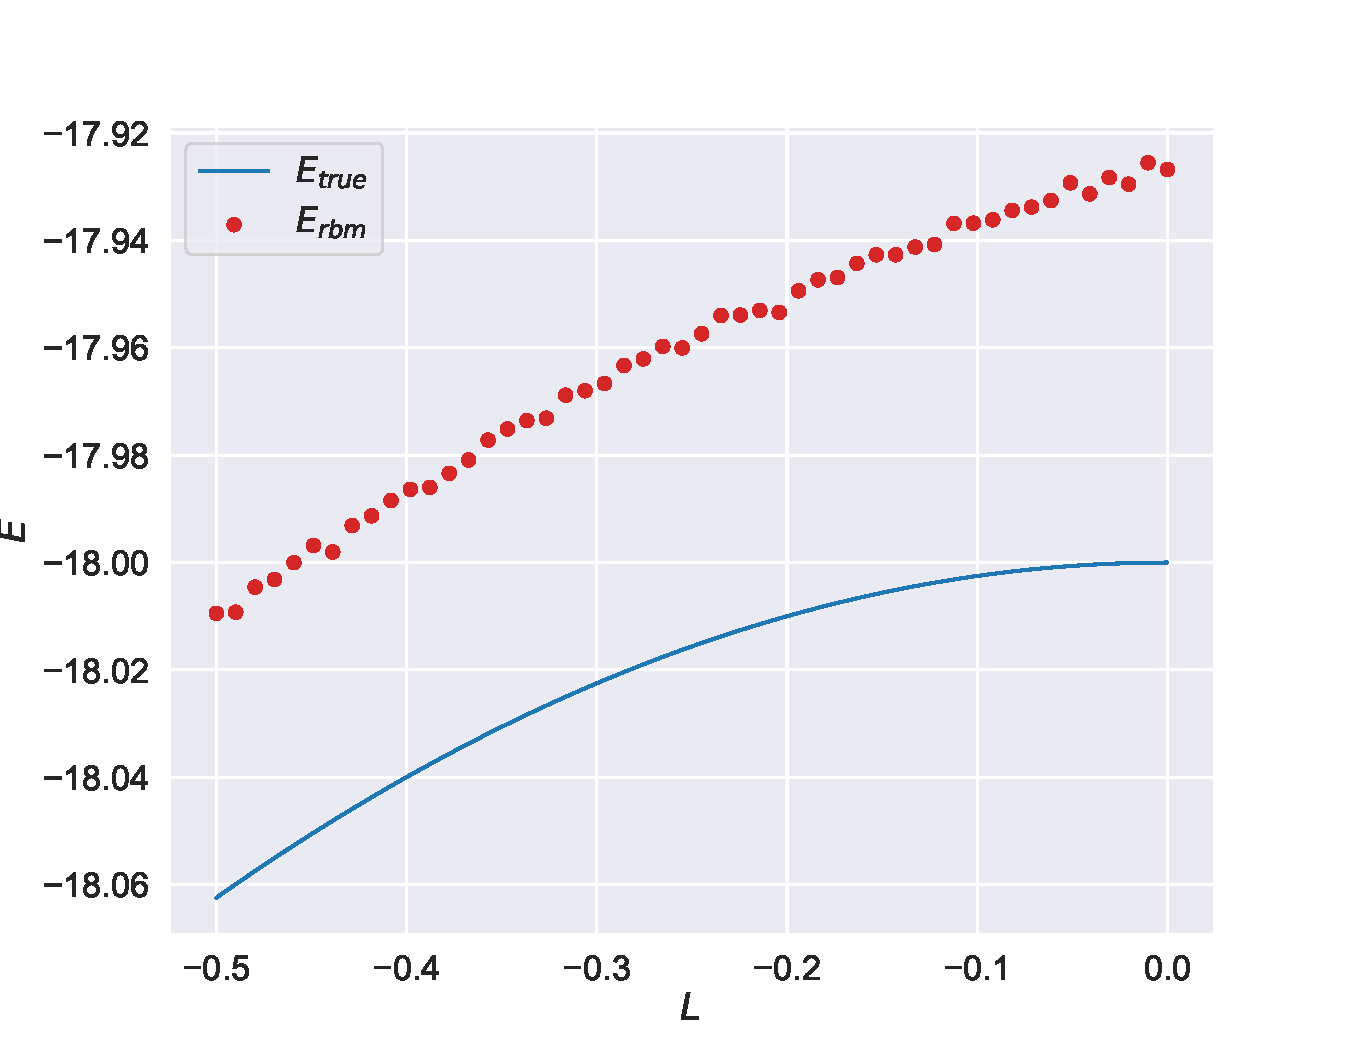
\includegraphics[width=0.95\textwidth]{Figures/Plots/Ising/val-true[L][-0.5-0.0][e=500][n=9][J=-1]}
  \end{center}
  \caption{The true ground state energy together with the restricted Boltzmann machine local energy output for the Ising model with $9$ lattice points, $N=3$ and $M=3$, and $J=-1$.}
\end{figure}

The RBM prediction doesn't quite line up with the true ground state energy, but the small scale of the y-axis means the actual error is not that large. We also still see the RBM prediction diverging away from the true ground state energy as the external field strength goes towards zero. From how the error evolved with the coupling strength variable one would expect the RBM to again default to a single basis state wavefunction too early again, but that is clearly not the case. 

